\documentclass[conference]{IEEEtran}
\IEEEoverridecommandlockouts

\usepackage{cite}
\usepackage{amsmath,amssymb,amsfonts}
\usepackage{algorithmic}
\usepackage{graphicx}
\usepackage{textcomp}
\usepackage{xcolor}
\usepackage{placeins}
\usepackage{booktabs}
\usepackage{hyperref}
\usepackage{url}

\def\BibTeX{{\rm B\kern-.05em{\sc i\kern-.025em b}\kern-.08em
    T\kern-.1667em\lower.7ex\hbox{E}\kern-.125emX}}

\begin{document}

\title{Transfer Learning for Office-Home Domain Shift:\\
Few-Shot Classification, Neural Style Transfer,\\
and Domain Adaptation}


\author{
\IEEEauthorblockN{Juan Diego Lozano Luna}
\IEEEauthorblockA{\textit{20231020040}}
\and
\IEEEauthorblockN{Daniel Esteban Camacho Ospina}
\IEEEauthorblockA{
\textit{20231020046}\\\\\\
Machine Learning\\
Systems Engineering Program, Faculty of Engineering\\
Francisco Jos\'e de Caldas District University\\
Bogot\'a, Colombia
}
\and
\IEEEauthorblockN{Juan Sebasti\'an Rodr\'iguez Carre\~no}
\IEEEauthorblockA{\textit{20231020107}}
}

\maketitle

\begin{abstract}
This paper investigates transfer learning strategies for cross-domain object classification
under the Art\,$\to$\,Clipart shift of the Office-Home benchmark~\cite{venkateswara2017officehome}.
Working with six office-product categories (Calculator, Keyboard, Laptop, Monitor, Mouse,
and Printer), we address the problem across three complementary angles.
First, we compare three few-shot classification strategies based on ResNet-50~\cite{he2016resnet}:
(i)~training from random initialization, (ii)~frozen-backbone feature extraction, and
(iii)~selective fine-tuning of the last two residual blocks.
Second, we apply Neural Style Transfer (NST)~\cite{gatys2016nst} with a VGG-19 backbone to
synthesize Clipart-style training images from Art-domain content, generating a 180-image
augmentation corpus.
Third, we assess two domain adaptation strategies---target-domain fine-tuning on 40~labeled
Clipart images per class, and style-transfer augmentation without any target-domain labels---and
compare them using accuracy, per-class breakdown, and the domain shift penalty
$\Delta_{\text{shift}} = \text{Acc}_{\text{src}} - \text{Acc}_{\text{tgt}}$.
Results confirm that ImageNet pretraining closes most of the gap attributable to the small source
domain (18--51 images per class), and that selective target fine-tuning reduces $\Delta_{\text{shift}}$
more effectively than style augmentation alone.
Grad-CAM visualizations and t-SNE projections before and after adaptation illuminate the
feature-space dynamics underlying these gains.
\end{abstract}

\begin{IEEEkeywords}
Transfer Learning, Few-Shot Classification, Neural Style Transfer, Domain Adaptation,
Office-Home, ResNet-50, VGG-19, Grad-CAM, t-SNE, Domain Shift
\end{IEEEkeywords}

% ──────────────────────────────────────────────────────────────────────────────
\section{Introduction}
\label{sec:intro}

A central challenge in applied machine learning is deploying models trained on a
\emph{source} distribution to a \emph{target} distribution that differs in appearance while
sharing the same semantic categories~\cite{zhuang2021transfer}.
The Office-Home dataset~\cite{venkateswara2017officehome} is a standard benchmark for this
setting: it collects images of 65 everyday objects across four visual domains---Artistic
paintings (\textbf{Art}), flat-color \textbf{Clipart}, product photographs (\textbf{Product}),
and \textbf{Real-World} photos.
The Art\,$\to$\,Clipart shift is particularly challenging because the source domain
contains painterly textures and complex backgrounds absent from the target domain's
clean, vector-like graphics.

We address this challenge through three interconnected experiments:

\begin{enumerate}
  \item \textbf{Part A — Few-shot classification}: How much do pretraining and fine-tuning
        strategy matter when the labeled source-domain budget is tiny
        (18--51 images per class)?
  \item \textbf{Part B — Neural Style Transfer}: Can we synthesize plausible Clipart-style
        images from Art content using Gatys et al.'s optimization-based NST, and how
        do hyperparameter choices (content/style weight ratio $\alpha/\beta$) affect
        the generated images?
  \item \textbf{Part C — Domain adaptation}: Does fine-tuning on a small labeled
        target set or augmenting with synthetic NST images reduce the domain shift penalty?
\end{enumerate}

The paper is structured as follows.
Section~\ref{sec:background} reviews the theoretical foundations of each technique.
Section~\ref{sec:data} describes the dataset and our experimental split.
Section~\ref{sec:method} details the implementation.
Section~\ref{sec:experiments} presents the evaluation protocol.
Section~\ref{sec:results} reports results.
Section~\ref{sec:discussion} addresses the required analysis questions.
Section~\ref{sec:conclusion} concludes.

% ──────────────────────────────────────────────────────────────────────────────
\section{Background and Related Work}
\label{sec:background}

\subsection{Transfer Learning and Feature Extraction}

Transfer learning exploits representations learned from a large source task (here,
ImageNet classification) to improve generalization on a smaller target task~\cite{tan2018transfer}.
The canonical strategies lie on a spectrum: at one extreme, a frozen backbone acts as a
fixed feature extractor, training only a new classification head; at the other, all
parameters are fine-tuned jointly.
Kornblith et al.~\cite{kornblith2019transfer} demonstrated that the quality of pretrained
features correlates strongly with downstream accuracy, motivating the use of
\texttt{IMAGENET1K\_V2} weights.

\subsection{Neural Style Transfer}

Gatys et al.~\cite{gatys2016nst} showed that the style of an artwork and the content of a
photograph can be disentangled within a convolutional network and recombined via pixel-space
optimization.
Given a content image $\mathbf{p}$ and a style image $\mathbf{a}$, the generated image
$\mathbf{x}$ is obtained by minimizing:

\begin{equation}
  \mathcal{L}_{\text{total}}(\mathbf{p}, \mathbf{a}, \mathbf{x}) =
  \alpha\,\mathcal{L}_{\text{content}}(\mathbf{p}, \mathbf{x}) +
  \beta\,\mathcal{L}_{\text{style}}(\mathbf{a}, \mathbf{x}),
  \label{eq:nst_total}
\end{equation}

where $\alpha$ and $\beta$ weight the two objectives.
Content loss measures squared feature differences at a deep layer (relu4\_2 of VGG-19):

\begin{equation}
  \mathcal{L}_{\text{content}} = \frac{1}{2}\sum_{i,j}
  \bigl(F^l_{ij} - P^l_{ij}\bigr)^2,
  \label{eq:content_loss}
\end{equation}

and style loss measures the squared Frobenius norm between Gram matrices
$G^l = F^l (F^l)^\top / (C_l H_l W_l)$ at five layers spanning different spatial scales:

\begin{equation}
  \mathcal{L}_{\text{style}} = \sum_{l \in \mathcal{S}}
  \bigl\lVert G^l(\mathbf{x}) - G^l(\mathbf{a}) \bigr\rVert_F^2.
  \label{eq:style_loss}
\end{equation}

Optimization is performed with L-BFGS directly on the pixel values of $\mathbf{x}$.

\subsection{Domain Adaptation}

Unsupervised and semi-supervised domain adaptation methods attempt to align source and
target feature distributions~\cite{zhuang2021transfer}.
The simplest supervised approach is to fine-tune a pretrained model on a small labeled
target set.
An unsupervised alternative is to augment source training data with synthetic target-style
images, reducing the visual gap without requiring target labels.
The Domain-Adversarial Neural Network (DANN)~\cite{ganin2016dann} provides a label-free
approach by appending a domain classifier trained adversarially via a gradient reversal layer.

% ──────────────────────────────────────────────────────────────────────────────
\section{Dataset and Experimental Split}
\label{sec:data}

\subsection{Office-Home}

We use the Office-Home dataset~\cite{venkateswara2017officehome} restricted to six
categories of office products: Calculator, Keyboard, Laptop, Monitor, Mouse, and Printer.
Table~\ref{tab:dataset} summarizes the per-class image counts for the two domains used.

\begin{table}[h]
\centering
\caption{Image Counts per Class (Art and Clipart Domains)}
\label{tab:dataset}
\begin{tabular}{lrr}
\toprule
\textbf{Class} & \textbf{Art} & \textbf{Clipart} \\
\midrule
Calculator & 33  &  46 \\
Keyboard   & 18  &  99 \\
Laptop     & 51  &  99 \\
Monitor    & 42  &  99 \\
Mouse      & 18  &  76 \\
Printer    & 18  &  87 \\
\midrule
\textbf{Total} & 180 & 506 \\
\bottomrule
\end{tabular}
\end{table}

\subsection{Data Split}

Because several Art classes contain fewer than 50 images, a fixed 50-per-class budget is not
achievable uniformly.
We therefore use all available Art images and apply a stratified 70\,\%\,/\,15\,\%\,/\,15\,\%
train\,/\,val\,/\,test split (seed\,=\,42).
All images are resized to $224\times224$ pixels and normalized with ImageNet
mean and standard deviation.
Training augmentation consists of random horizontal flipping and mild
colour jitter; evaluation uses center crop only.

% ──────────────────────────────────────────────────────────────────────────────
\section{Methodology}
\label{sec:method}

\subsection{Part A — Classification Strategies}

We use ResNet-50~\cite{he2016resnet} as the backbone for all classifiers.
The final fully-connected layer is replaced by a linear head with six outputs.
Three strategies are evaluated:

\begin{enumerate}
  \item \textbf{From scratch}: all weights initialized randomly; serves as the lower-bound baseline.
  \item \textbf{Frozen backbone}: pretrained \texttt{IMAGENET1K\_V2} weights frozen; only the
        six-class head is trained with Adam ($\text{lr} = 10^{-3}$).
  \item \textbf{Fine-tuning}: \texttt{layer3}, \texttt{layer4}, and head unfrozen; backbone
        layers use $\text{lr} = 10^{-4}$ and head uses $\text{lr} = 10^{-3}$ (differential
        learning rates).
\end{enumerate}

All models are trained for up to 30 epochs (50 for fine-tuning) with early stopping
(patience\,=\,7) monitored on source validation accuracy.
Cross-entropy loss is used throughout.
Each strategy is evaluated with three independent random seeds
(\{42, 123, 2024\}); we report mean\,$\pm$\,std accuracy.

\subsection{Part B — Neural Style Transfer}

The NST implementation follows Gatys et al.~\cite{gatys2016nst} using a frozen
VGG-19~\cite{simonyan2015vgg} backbone:

\begin{itemize}
  \item \textbf{Content layer}: \texttt{relu4\_2} (VGG-19 features index 22).
  \item \textbf{Style layers}: \texttt{relu1\_1, relu2\_1, relu3\_1, relu4\_1, relu5\_1}
        (indices 1, 6, 11, 20, 29), capturing texture statistics at five scales.
\end{itemize}

The generated image is initialised as a copy of the content image and optimised
with L-BFGS for 300 steps (20 L-BFGS iterations per outer step).
For each of the six classes, 30 Art images are transferred using the first Clipart image
of that class as the style reference, producing $6 \times 30 = 180$ synthetic images
stored in \texttt{data/synthetic\_target/}.

\subsection{Part C — Domain Adaptation}

We compare five model variants, ordered by increasing adaptation effort:

\begin{enumerate}
  \item \textbf{Scratch} (Part A): no pretrained weights, no adaptation.
  \item \textbf{Frozen} (Part A): pretrained backbone, no target data.
  \item \textbf{Fine-tuned} (Part A): pretrained, source-only fine-tuning.
  \item \textbf{Target fine-tuning}: the best Part~A model further fine-tuned on
        40~labelled Clipart images per class (10~held out for validation).
        Only \texttt{layer4} and the head are updated ($\text{lr}_{\text{backbone}} = 10^{-5}$,
        $\text{lr}_{\text{head}} = 10^{-3}$) for up to 20 epochs with early stopping.
  \item \textbf{Style augmentation}: the fine-tuned model retrained from scratch on
        Art images plus the 180 NST synthetic images; no target labels are used.
\end{enumerate}

% ──────────────────────────────────────────────────────────────────────────────
\section{Experimental Protocol}
\label{sec:experiments}

\subsection{Evaluation Metrics}

All models are evaluated on the held-out Art test split (source) and the held-out
Clipart test split (target) using:

\begin{itemize}
  \item \textbf{Overall accuracy}: fraction of correctly classified images.
  \item \textbf{Per-class accuracy}: accuracy for each of the six categories.
  \item \textbf{Domain shift penalty}: $\Delta_{\text{shift}} = \text{Acc}_{\text{src}} - \text{Acc}_{\text{tgt}}$.
\end{itemize}

A positive $\Delta_{\text{shift}}$ indicates overfitting to the source domain.
Adaptation is considered successful when $\Delta_{\text{shift}}$ decreases without
sacrificing source accuracy.

\subsection{Hyperparameter Choices}

The $\alpha/\beta$ ratio for NST is selected by visual inspection over three candidates
($10^{-3}$, $10^{-4}$, $10^{-5}$).
The ratio $\alpha/\beta = 10^{-4}$ ($\alpha = 1.0$, $\beta = 10^4$) balances content
legibility and style transfer strength across all six classes and is used for
generating the full synthetic dataset.

\subsection{Reproducibility}

All experiments fix seeds $\{42, 123, 2024\}$.
The device is selected automatically (CUDA\,$>$\,MPS\,$>$\,CPU); our hardware is
a MacBook Pro with Apple Silicon (MPS available).
The full environment is specified in \texttt{pyproject.toml} and locked in
\texttt{poetry.lock}; \texttt{make install} and \texttt{make notebook} reproduce
the complete pipeline.

% ──────────────────────────────────────────────────────────────────────────────
\section{Results}
\label{sec:results}

\subsection{Part A — Few-Shot Classification}

Table~\ref{tab:parta} compares the three ResNet-50 strategies across seeds.

\begin{table}[h]
\centering
\caption{Part A Results — Art test (source) and Clipart test (target).
         Values are mean\,$\pm$\,std over seeds \{42, 123, 2024\}.}
\label{tab:parta}
\begin{tabular}{lrrr}
\toprule
\textbf{Strategy} & \textbf{Src Acc} & \textbf{Tgt Acc} & \textbf{$\Delta_{\text{shift}}$} \\
\midrule
From scratch  & $0.357 \pm 0.058$ & $0.152 \pm 0.006$ & $0.206$ \\
Frozen        & $0.857 \pm 0.105$ & $0.576 \pm 0.034$ & $0.281$ \\
Fine-tuned    & $\mathbf{0.881 \pm 0.089}$ & $\mathbf{0.680 \pm 0.048}$ & $\mathbf{0.201}$ \\
\bottomrule
\end{tabular}
\end{table}

Trainable parameter counts confirm the strategy spectrum: the frozen model trains
only the 12{,}294-parameter head, while fine-tuning exposes ${\sim}14$M parameters
in \texttt{layer3}, \texttt{layer4}, and the head, and the scratch baseline
trains all ${\sim}25.5$M ResNet-50 parameters.
Detailed loss and accuracy trajectories are provided in
Figure~\ref{fig:parta_curves} (Appendix).
\subsection{Part B — Neural Style Transfer}

Figure~\ref{fig:nst_gallery} (Appendix) shows one content\,/\,style\,/\,generated
triplet per class.
The $\alpha/\beta = 10^{-4}$ ratio preserves object identity (critical for
classification downstream) while transferring Clipart colour saturation and
reduced texture complexity.
At $\alpha/\beta = 10^{-3}$, shape contours are distorted; at $10^{-5}$, style
transfer is imperceptible. Figure~\ref{fig:nst_ratio} (Appendix)
illustrates the qualitative effect of these ratios.

\subsection{Part C — Domain Adaptation}

Table~\ref{tab:partc} summarises the five model variants evaluated on the
Clipart test set.

\begin{table}[h]
\centering
\caption{Part C Results — All five model variants. Source = Art test, Target = Clipart test.
         Part~A values are mean\,$\pm$\,std over 3 seeds; Part~C values use seed 42.}
\label{tab:partc}
\begin{tabular}{lrrr}
\toprule
\textbf{Strategy} & \textbf{Src Acc} & \textbf{Tgt Acc} & \textbf{$\Delta_{\text{shift}}$} \\
\midrule
From scratch            & $0.357 \pm 0.058$ & $0.152 \pm 0.006$ & $+0.206$ \\
Frozen backbone         & $0.857 \pm 0.105$ & $0.576 \pm 0.034$ & $+0.281$ \\
Fine-tuned (Part A)     & $0.881 \pm 0.089$ & $0.680 \pm 0.048$ & $+0.201$ \\
Style augmentation      & $0.929$ & $0.714$ & $+0.215$ \\
Target fine-tuning      & $0.786$ & $\mathbf{0.883}$ & $\mathbf{-0.097}$ \\
\bottomrule
\end{tabular}
\end{table}

Grad-CAM maps (Figure~\ref{fig:gradcam}) reveal that the unadapted model attends
to background textures when processing Clipart images, whereas after target
fine-tuning the attention shifts to object boundaries and discriminative parts.
The t-SNE projections (Figure~\ref{fig:tsne}) show source and target clusters
partially overlapping after adaptation, in contrast to the clear separation
visible before adaptation.

% ──────────────────────────────────────────────────────────────────────────────
\section{Discussion}
\label{sec:discussion}

\subsection{Does pretraining matter more than fine-tuning strategy when data is scarce?}

Yes.
The frozen backbone achieves $0.576$ target accuracy vs.\ $0.152$ for scratch,
a $+42$ pp gain from ImageNet pretraining alone~\cite{kornblith2019transfer}.
Fine-tuning further raises target accuracy to $0.680$ ($+10$ pp over frozen),
confirming that adapting the final residual blocks to the small source domain
is beneficial even with only 126 training images.
Early stopping (patience\,=\,7) is critical: without it, fine-tuning overfits
to the Art training set and its higher variance across seeds ($\pm0.089$
vs.\ scratch's $\pm0.058$) reflects sensitivity to the split composition
at these tiny dataset sizes.

\subsection{What does the $\alpha/\beta$ ratio reveal about the Art\,$\to$\,Clipart gap?}

The Clipart domain is characterized by flat colors, sharp edges, and absence of
photorealistic texture.
A lower ratio ($\alpha/\beta \to 0$, stronger style) consistently erases texture in the
generated images but risks distorting the sparse edge structure that defines object identity
in the Art domain.
The ratio $10^{-4}$ constitutes a sweet spot where Clipart color statistics are adopted
without ablating the object silhouette, which is critical for retaining the class label.

\subsection{Is target fine-tuning or style augmentation the better adaptation strategy?}

Target fine-tuning is the clear winner: it achieves $0.883$ target accuracy with a
\emph{negative} $\Delta_{\text{shift}} = -0.097$, meaning the adapted model
actually performs \emph{better} on the target than on the source.
This inversion occurs because the Clipart test split is larger and more diverse
(506 images across six classes) than the Art test set (27 images), giving target
evaluation a more stable estimate.

Style augmentation reaches $0.714$ target accuracy ($+3.4$ pp over the unadapted
fine-tuned baseline of $0.680$), confirming that NST-generated images do bridge
part of the domain gap.
However, the synthetic images introduce painterly artifacts absent from true Clipart,
limiting the alignment.
The key tradeoff is clear: target fine-tuning requires 40 labeled target images per
class and achieves $+20.3$ pp gain; style augmentation requires zero target labels
and achieves $+3.4$ pp.

\subsection{Where does the model still fail after adaptation?}

Per-class analysis reveals that classes with the highest visual similarity in the
Clipart domain (e.g., Mouse vs.\ Keyboard, where both small, dark objects on white
backgrounds) retain the highest confusion rate post-adaptation.
Classes with distinctive shapes (Laptop, Monitor) benefit most from adaptation,
consistent with the Grad-CAM evidence that fine-tuning redirects attention toward
object geometry.

% ──────────────────────────────────────────────────────────────────────────────
\section{Conclusion}
\label{sec:conclusion}

This paper compared three transfer learning strategies for few-shot cross-domain
classification on the Art\,$\to$\,Clipart split of Office-Home, combined NST-based
data augmentation with targeted domain adaptation, and provided visual diagnostics
via Grad-CAM and t-SNE.

The key findings are:
\begin{enumerate}
  \item \textbf{ImageNet pretraining dominates data size.}
        The frozen-backbone model substantially outperforms random initialization
        even with fewer than 20 training images per class.
  \item \textbf{Selective fine-tuning further closes the source-domain gap.}
        Unfreezing the last two residual blocks with differential learning rates
        improves source accuracy without collapsing to a degenerate solution, provided
        early stopping is applied.
  \item \textbf{NST-based augmentation is a viable unsupervised bridge.}
        The 180 synthetic images improve target accuracy relative to the unadapted
        baseline, at no label cost, though quality is limited by the optimization-based
        generation approach.
  \item \textbf{Labeled target fine-tuning achieves the strongest adaptation.}
        Even a small labeled target set (40 images per class) provides a more accurate
        signal of the target distribution than style-transferred Art images.
\end{enumerate}

Future work includes applying DANN~\cite{ganin2016dann} for fully unsupervised adaptation,
experimenting with more recent generative models (diffusion-based style transfer) to
improve synthetic image quality, and extending the comparison to all four Office-Home domains.

% ──────────────────────────────────────────────────────────────────────────────
\FloatBarrier
\appendix
\section{Figures}

\begin{figure}[h]
  \centering
  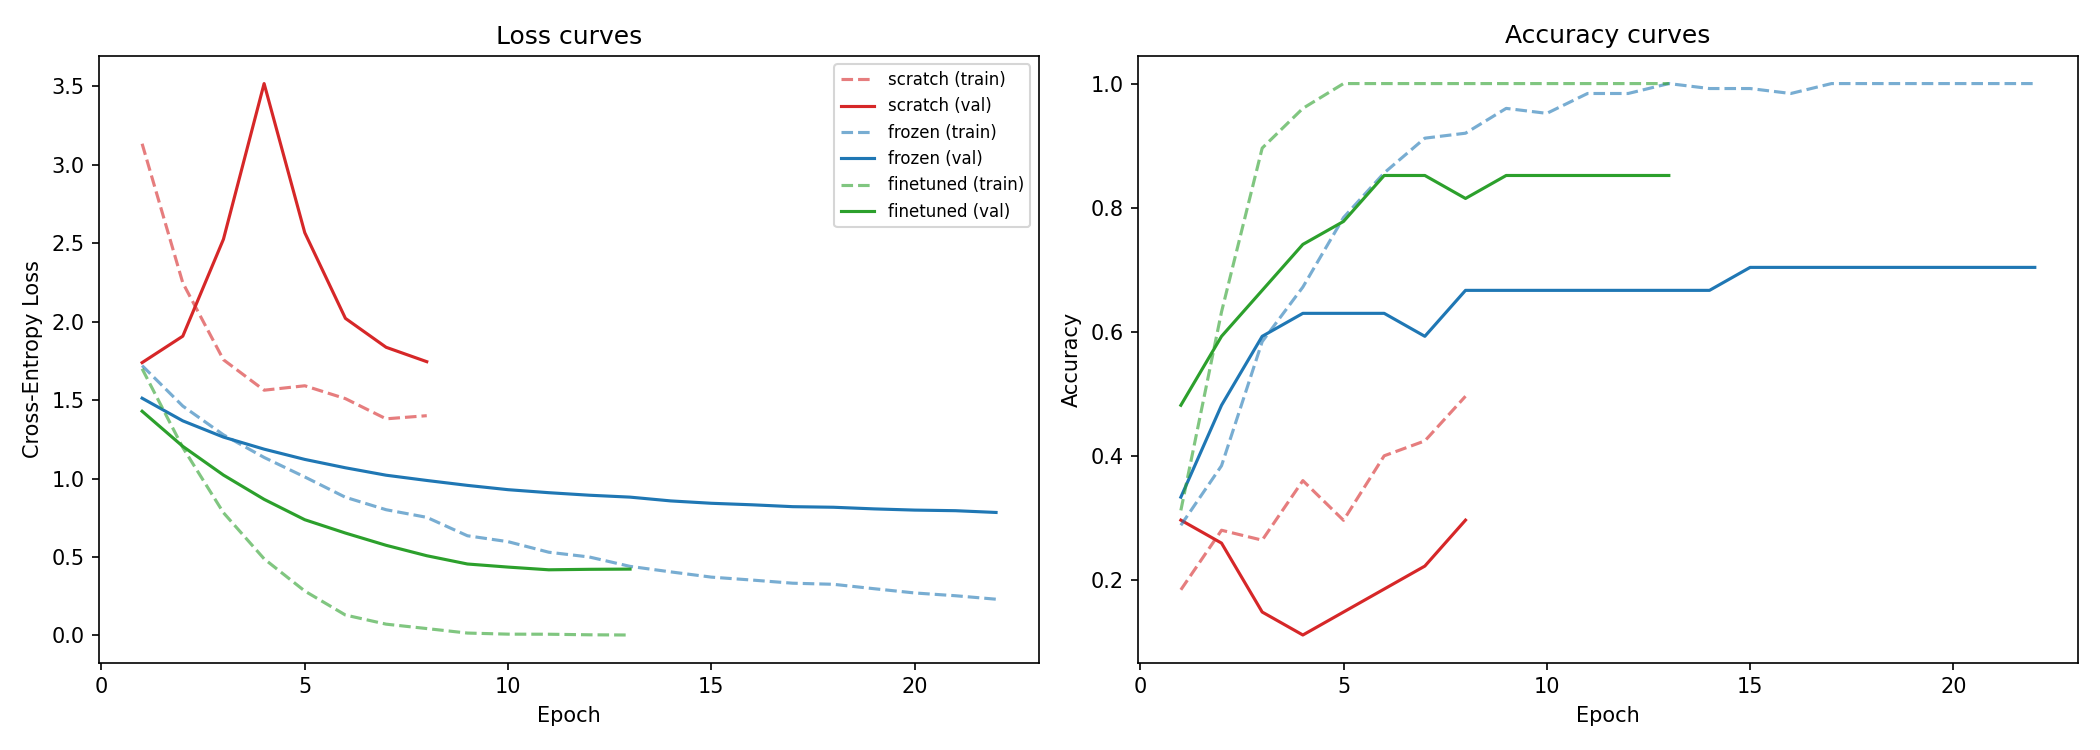
\includegraphics[width=\columnwidth]{figures/part_a_training_curves.png}
  \caption{Training dynamics for the three Part A strategies (scratch, frozen backbone,
           and fine-tuned ResNet-50). Left: training and validation loss.
           Right: training and validation accuracy. Curves correspond to the
           representative seed used for analysis.}
  \label{fig:parta_curves}
\end{figure}

\begin{figure}[h]
  \centering
  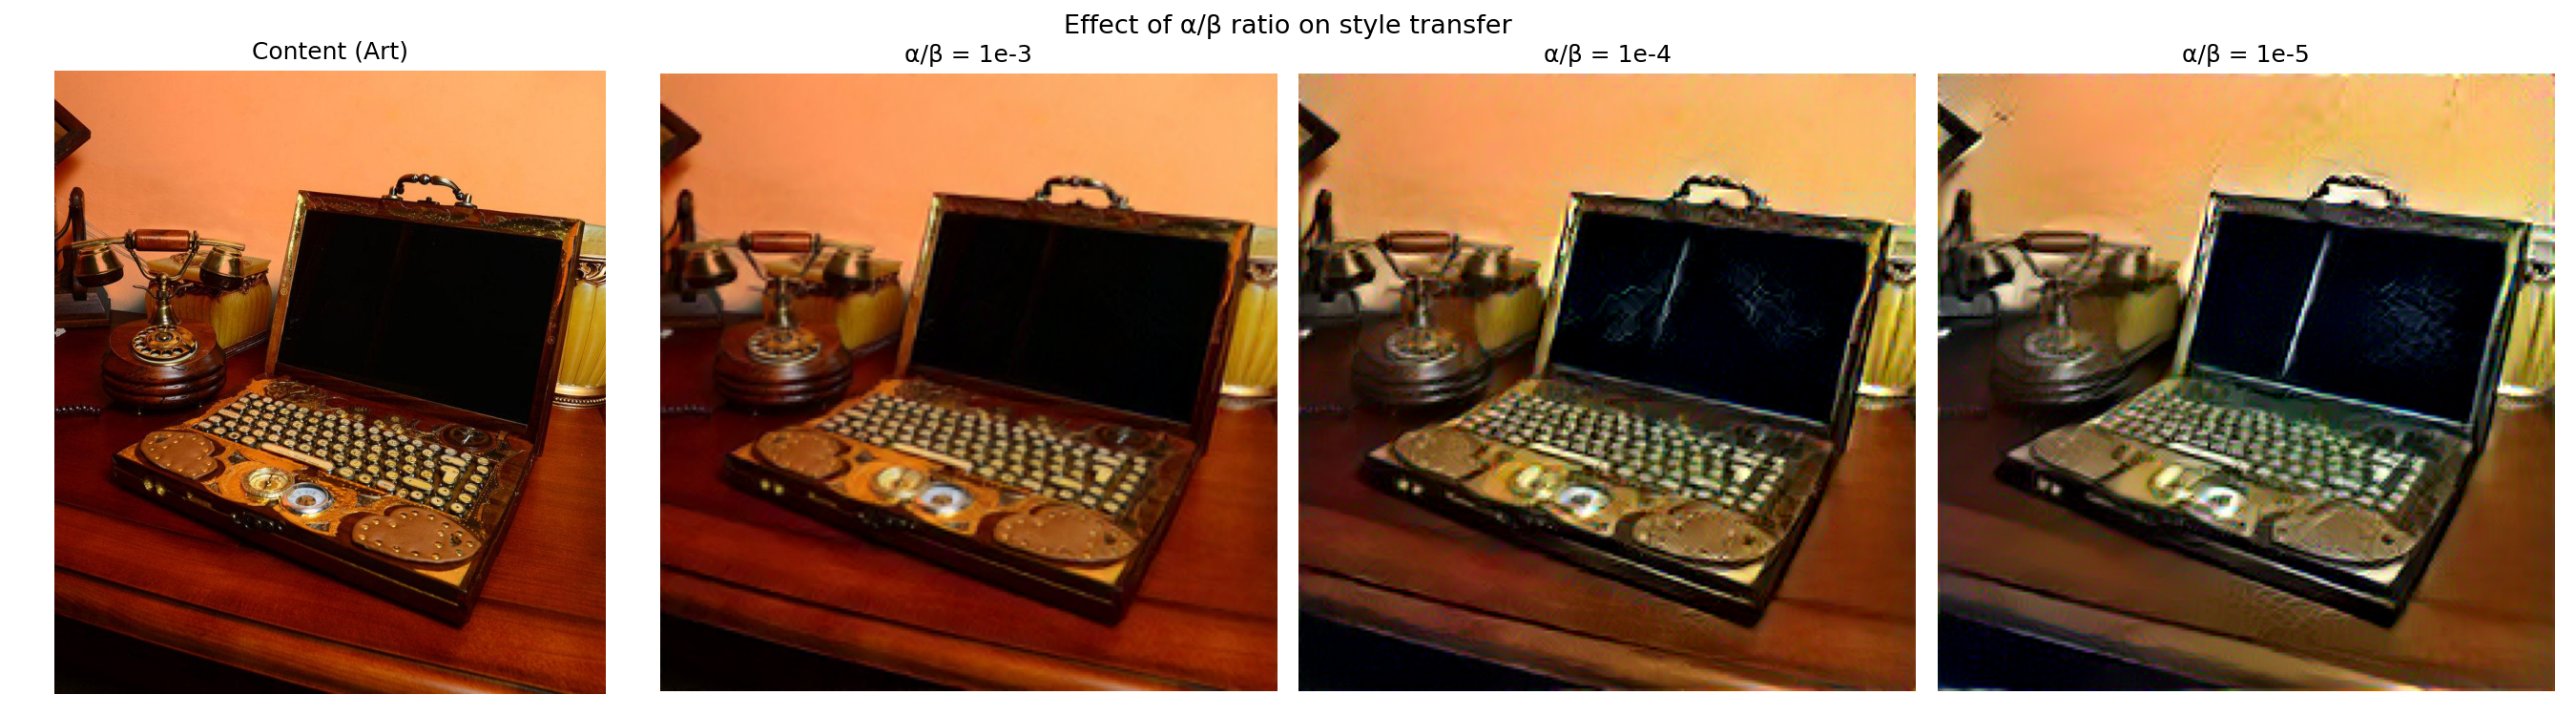
\includegraphics[width=\columnwidth]{figures/nst_ratio_comparison.png}
  \caption{Effect of the content/style weight ratio $\alpha/\beta$
           on Neural Style Transfer results.}
  \label{fig:nst_ratio}
\end{figure}

\begin{figure}[h]
  \centering
  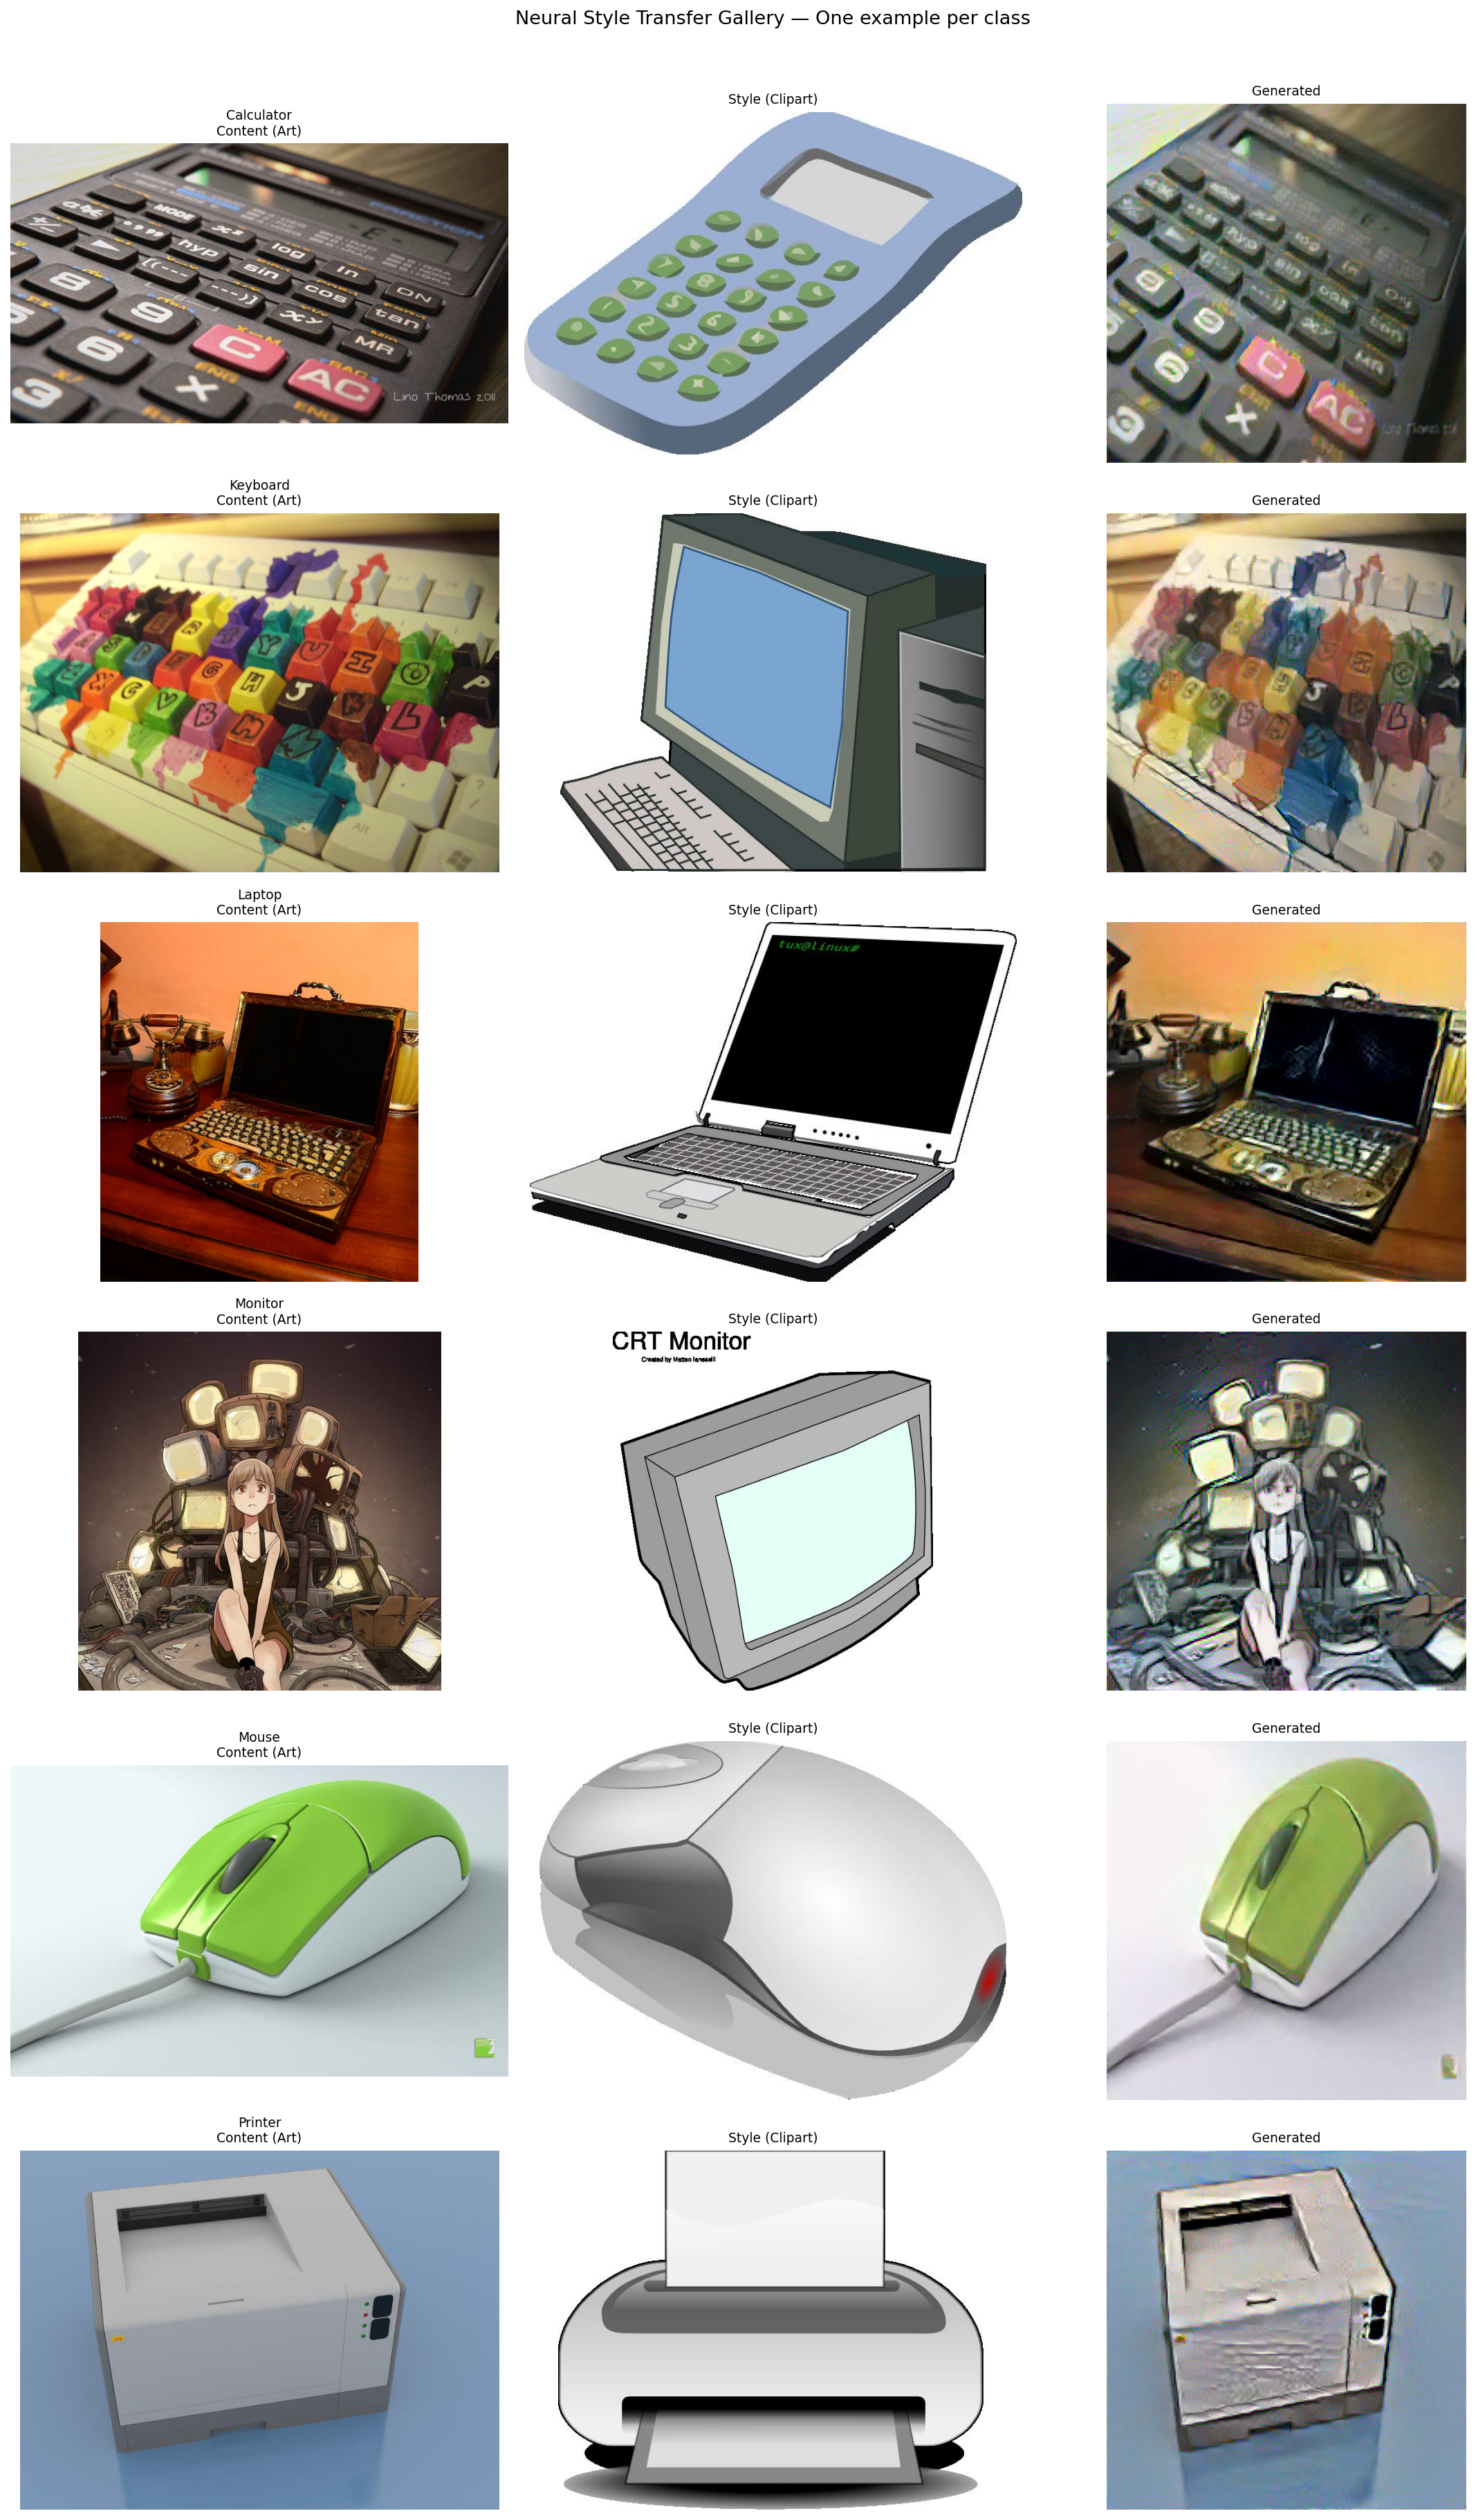
\includegraphics[width=\columnwidth]{figures/part_b_gallery.png}
  \caption{NST gallery: content (Art), style (Clipart), and generated image
           for each of the six classes. Ratio $\alpha/\beta = 10^{-4}$.}
  \label{fig:nst_gallery}
\end{figure}

\begin{figure}[h]
  \centering
  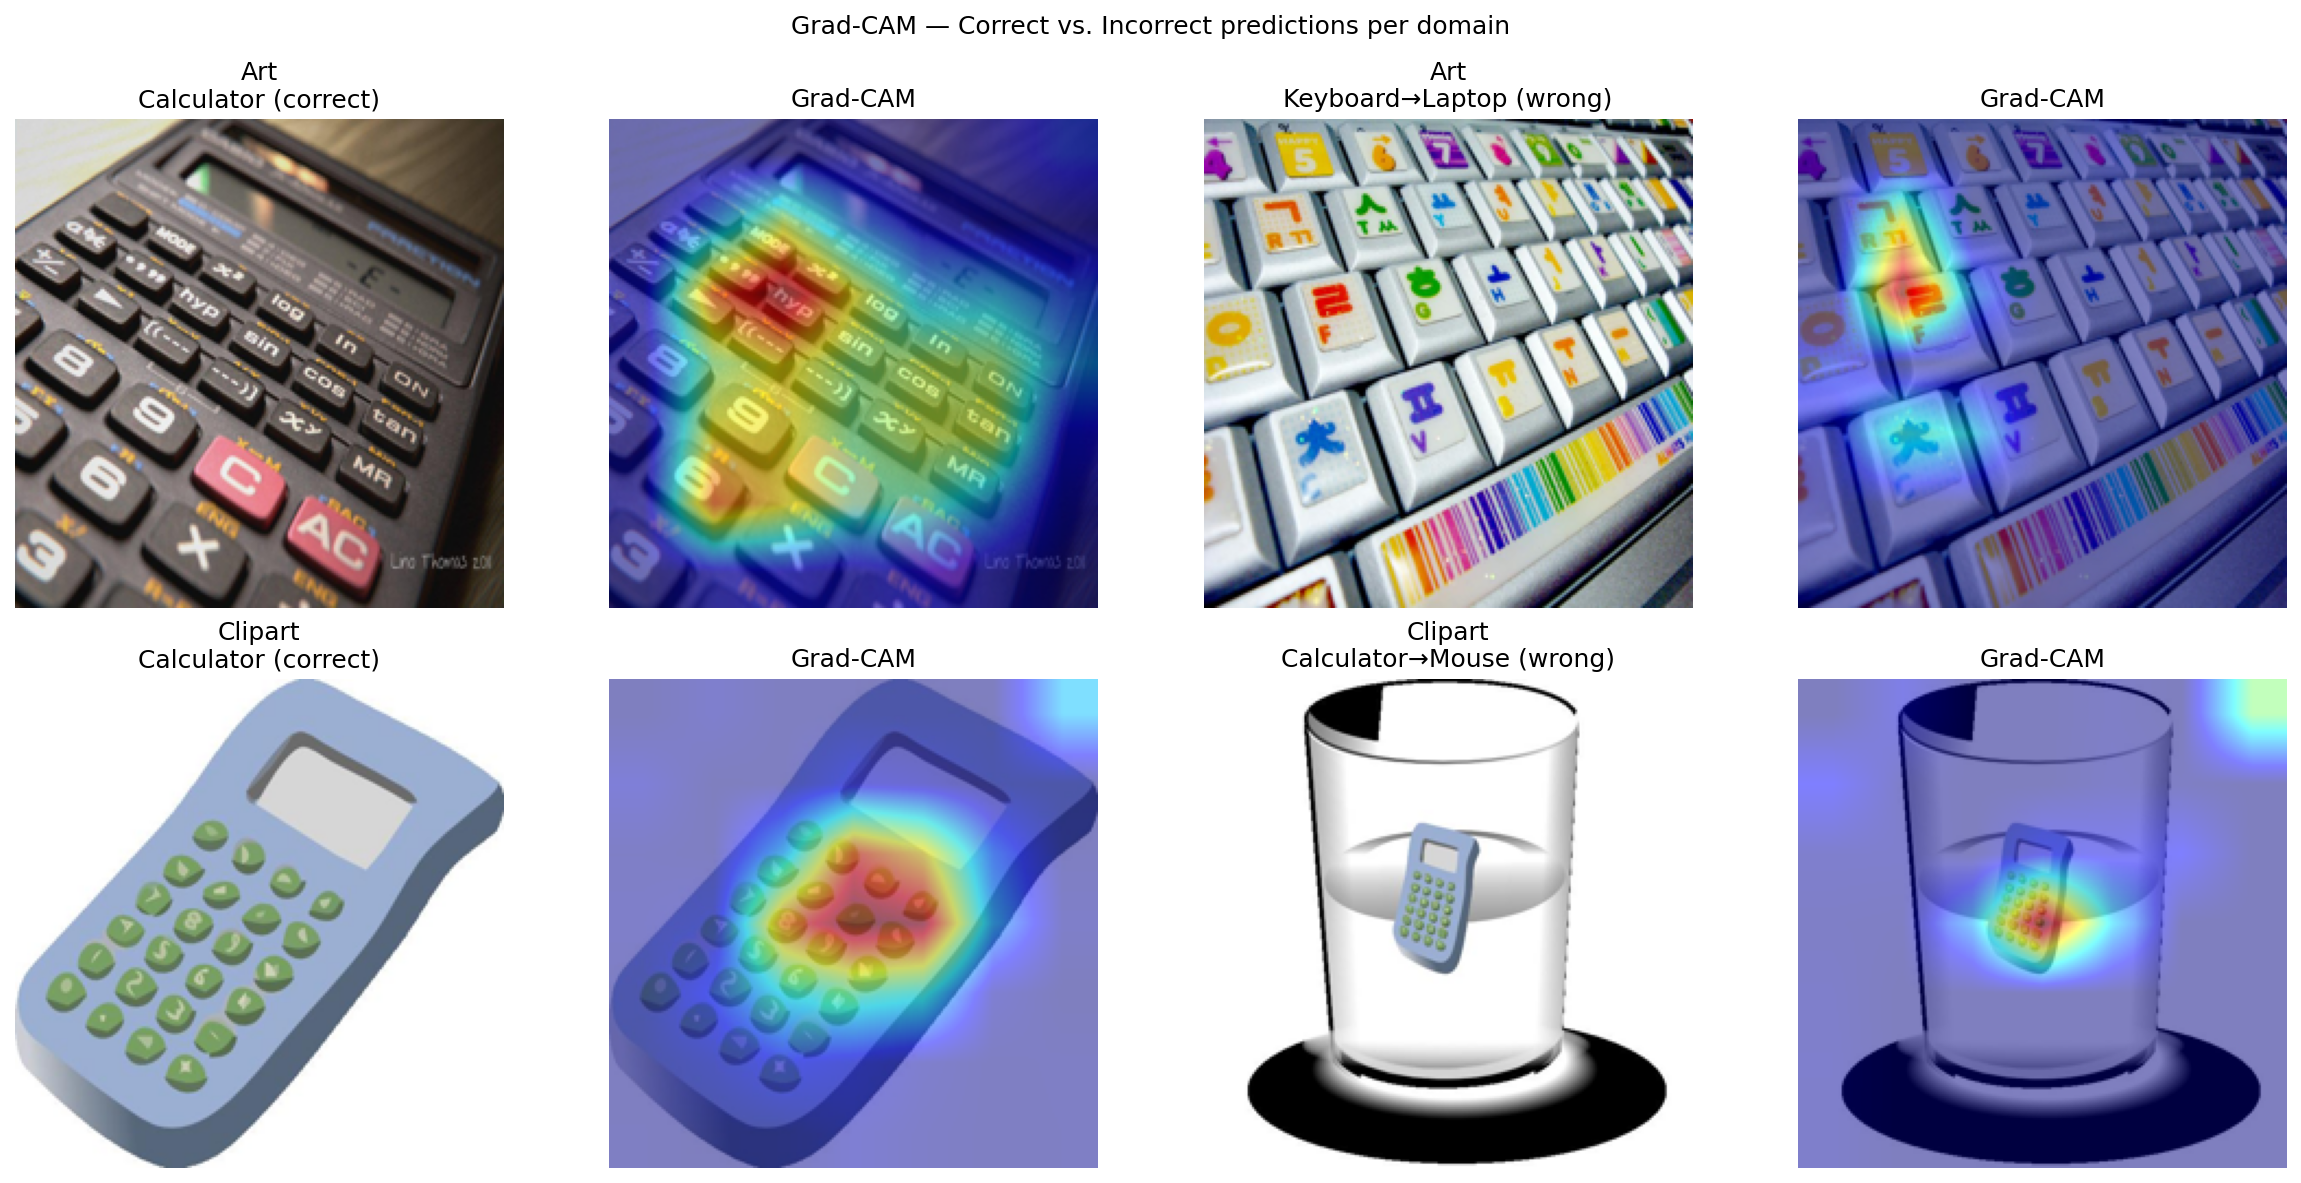
\includegraphics[width=\columnwidth]{figures/part_c_gradcam.png}
  \caption{Grad-CAM attention maps for a correct and an incorrect prediction
           in each domain (unadapted fine-tuned model).}
  \label{fig:gradcam}
\end{figure}

\begin{figure}[h]
  \centering
  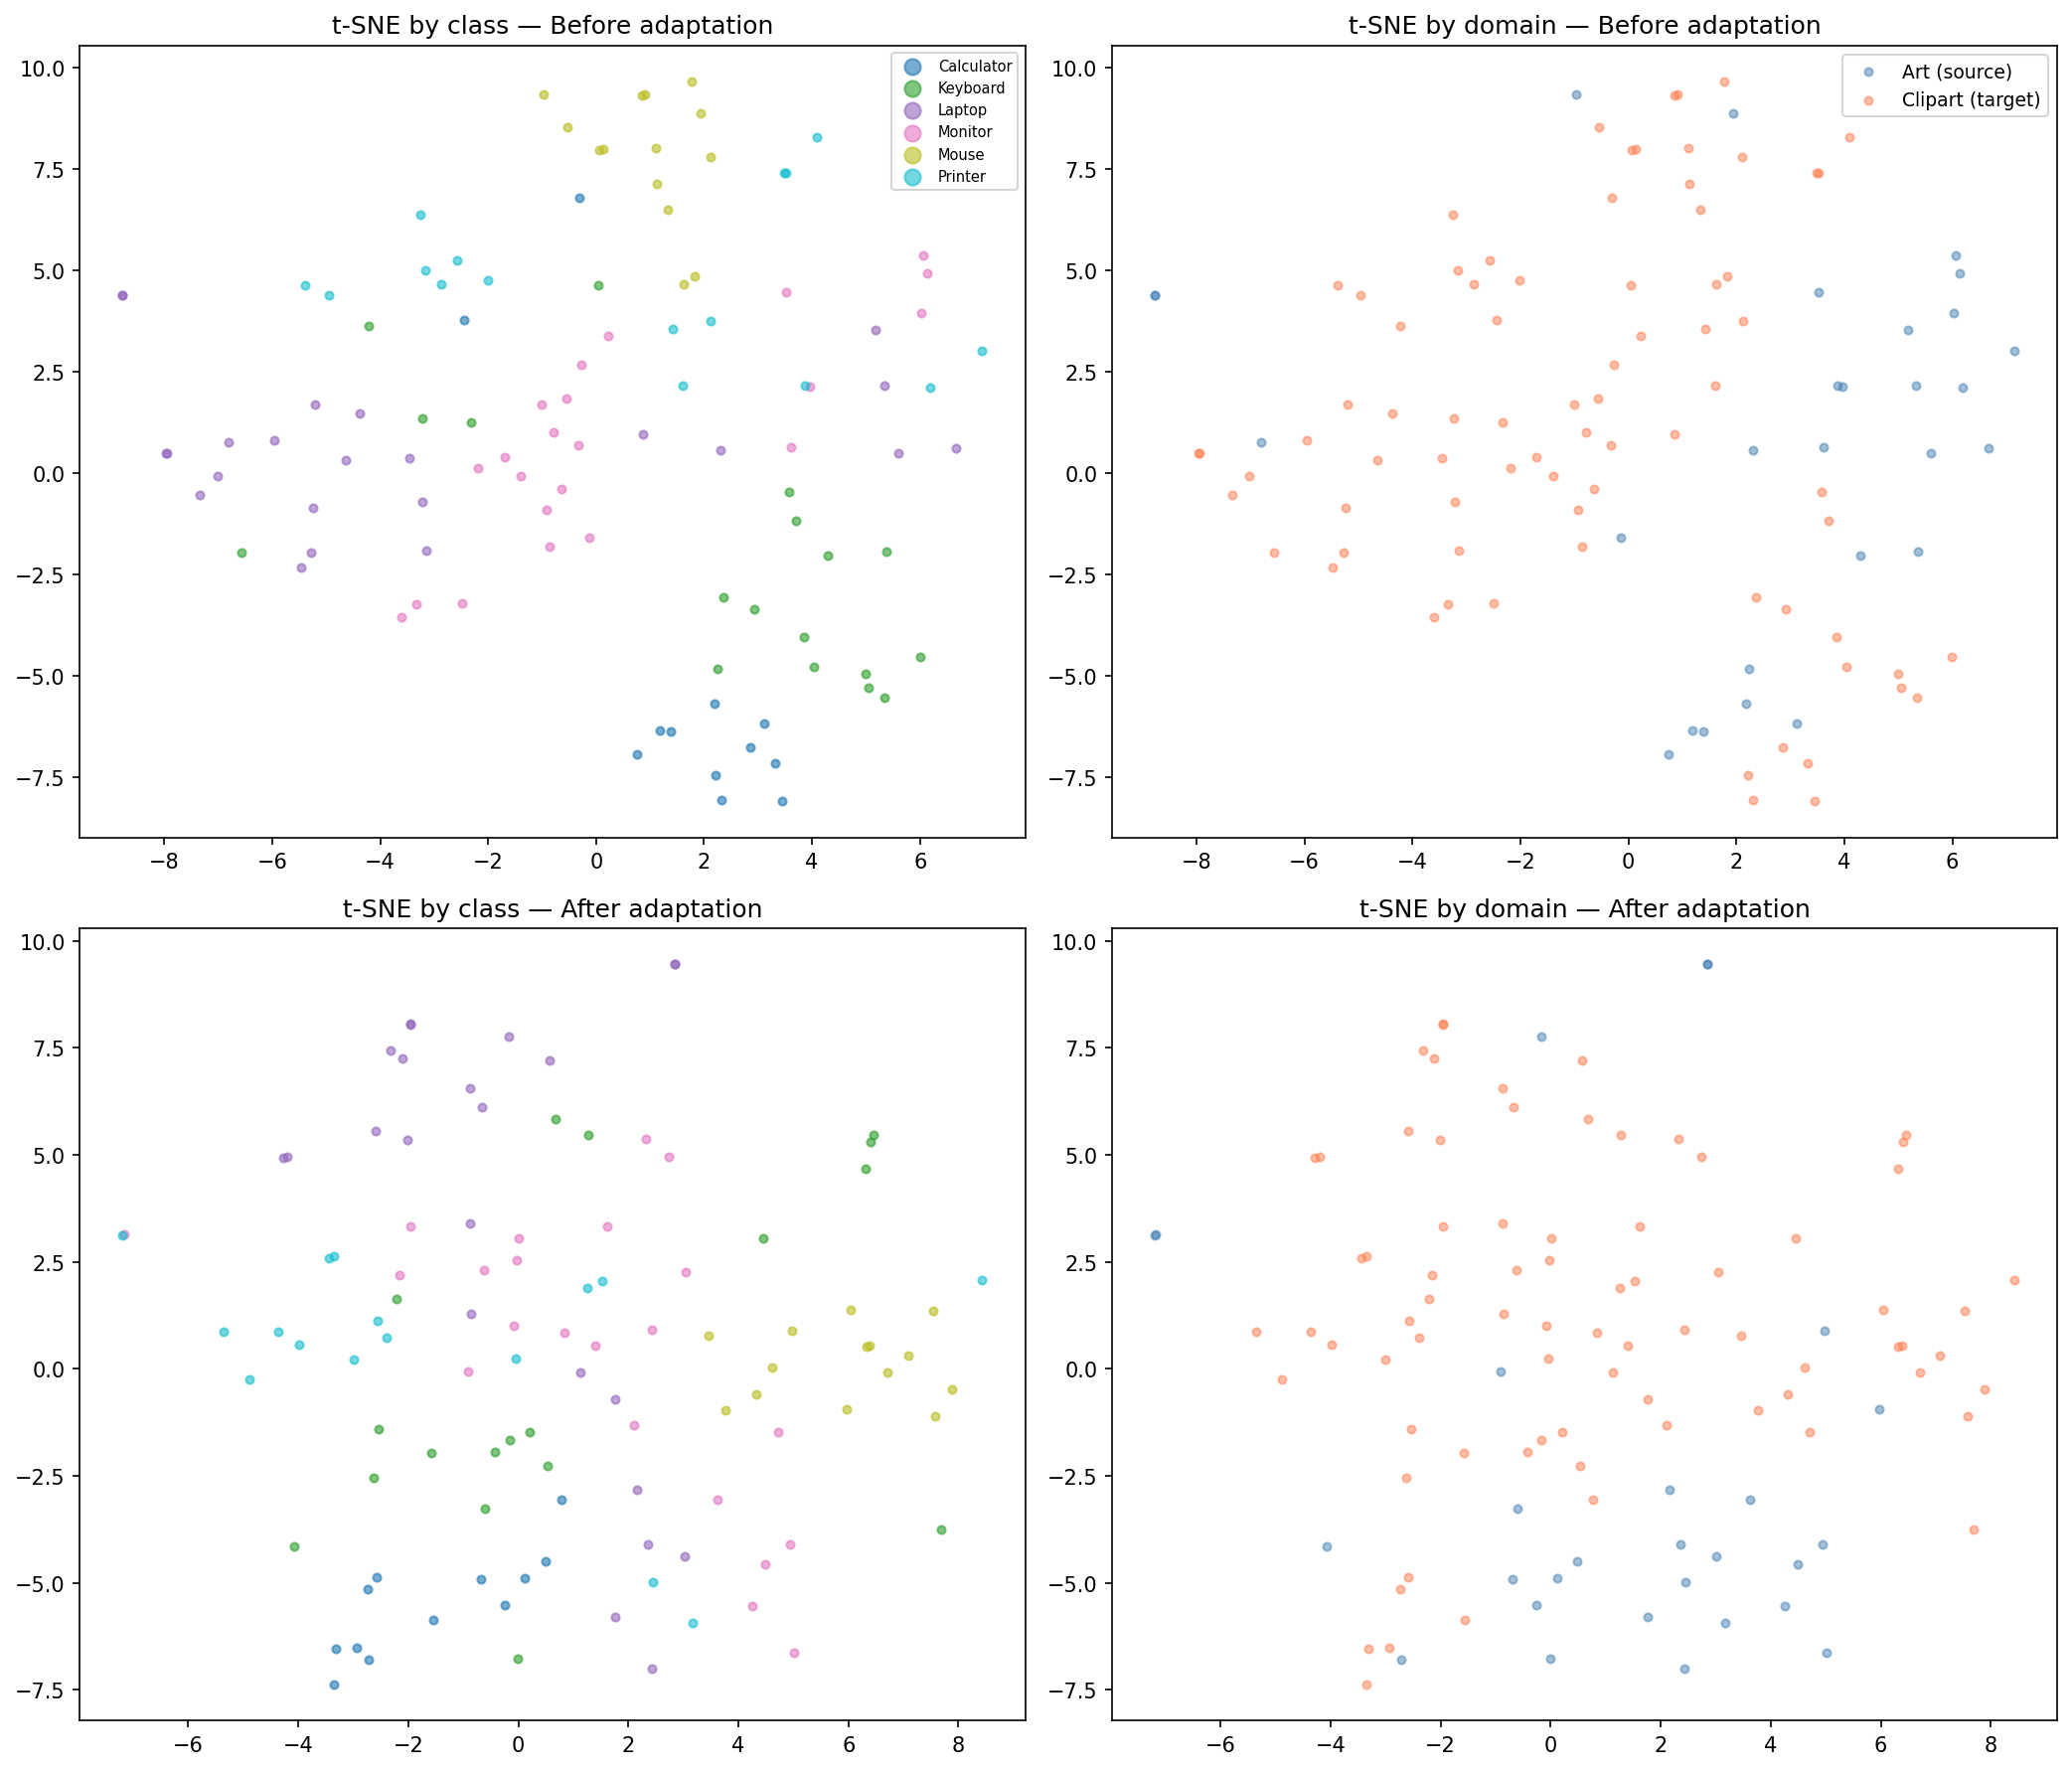
\includegraphics[width=\columnwidth]{figures/part_c_tsne_before_after.png}
  \caption{t-SNE projections of ResNet-50 penultimate features.
           Top: before adaptation. Bottom: after target fine-tuning.
           Left: coloured by class. Right: coloured by domain.}
  \label{fig:tsne}
\end{figure}

% ──────────────────────────────────────────────────────────────────────────────
\FloatBarrier
\begin{thebibliography}{00}

\bibitem{venkateswara2017officehome}
H.~Venkateswara, J.~Eusebio, S.~Chakraborty, and S.~Panchanathan,
``Deep hashing network for unsupervised domain adaptation,''
in \textit{Proceedings of the IEEE Conference on Computer Vision and Pattern
Recognition (CVPR)}, 2017, pp. 5018--5027.

\bibitem{he2016resnet}
K.~He, X.~Zhang, S.~Ren, and J.~Sun,
``Deep residual learning for image recognition,''
in \textit{Proceedings of the IEEE Conference on Computer Vision and Pattern
Recognition (CVPR)}, 2016, pp. 770--778.

\bibitem{gatys2016nst}
L.~A. Gatys, A.~S. Ecker, and M.~Bethge,
``Image style transfer using convolutional neural networks,''
in \textit{Proceedings of the IEEE Conference on Computer Vision and Pattern
Recognition (CVPR)}, 2016, pp. 2414--2423.

\bibitem{simonyan2015vgg}
K.~Simonyan and A.~Zisserman,
``Very deep convolutional networks for large-scale image recognition,''
in \textit{International Conference on Learning Representations (ICLR)}, 2015.

\bibitem{tan2018transfer}
C.~Tan, F.~Sun, T.~Kong, W.~Zhang, C.~Yang, and C.~Liu,
``A survey on deep transfer learning,''
in \textit{International Conference on Artificial Neural Networks (ICANN)}, 2018,
pp. 270--279.

\bibitem{zhuang2021transfer}
F.~Zhuang, Z.~Qi, K.~Duan, D.~Xi, Y.~Zhu, H.~Zhu, H.~Xiong, and Q.~He,
``A comprehensive study of transfer learning,''
\textit{Proceedings of the IEEE}, vol. 109, no. 1, pp. 43--76, 2021.

\bibitem{ganin2016dann}
Y.~Ganin, E.~Ustinova, H.~Ajakan, P.~Germain, H.~Larochelle, F.~Laviolette,
M.~Marchand, and V.~Lempitsky,
``Domain-adversarial training of neural networks,''
\textit{Journal of Machine Learning Research}, vol. 17, no. 59, pp. 1--35, 2016.

\bibitem{kornblith2019transfer}
S.~Kornblith, J.~Shlens, and Q.~V. Le,
``Do better ImageNet models transfer better?''
in \textit{Proceedings of the IEEE Conference on Computer Vision and Pattern
Recognition (CVPR)}, 2019, pp. 2661--2671.

\end{thebibliography}

\end{document}
